\documentclass[conference]{IEEEtran}
\usepackage{cite}
\usepackage{amsmath,amssymb,amsfonts}
\usepackage{algorithmic}
\usepackage{graphicx}
\usepackage{textcomp}
\usepackage{xcolor}
\usepackage{booktabs}
\usepackage{url}
\usepackage{array}
\usepackage{siunitx}

\begin{document}

\title{Privacy--Heterogeneity Trade-offs and Contribution Valuation in Scalable Federated Prostate Cancer Staging}

\author{\IEEEauthorblockN{Ponnaluri Jeyanth}
\IEEEauthorblockA{\textit{CSE (Data Science)} \\
\textit{R.V.R. \& J.C. College of Engineering}\\
Guntur, India \\
jeyanthponnaluri08@gmail.com}
\and
\IEEEauthorblockN{Pudota Jaideep}
\IEEEauthorblockA{\textit{CSE (Data Science)} \\
\textit{R.V.R. \& J.C. College of Engineering}\\
Guntur, India \\
pudotajaideep@gmail.com}
\and
\IEEEauthorblockN{Dr. M.V.P. Chandra Sekhara Rao}
\IEEEauthorblockA{\textit{Professor \& Head, CSE (DS)} \\
\textit{R.V.R. \& J.C. College of Engineering}\\
Guntur, India \\
manukondach@gmail.com}
}

\maketitle

\begin{abstract}
Collaborative machine learning in medical networks is hindered by strict data privacy regulations and statistical heterogeneity across clinical sites. While federated learning enables multi-institutional training, the multi-dimensional interactions between statistical heterogeneity and privacy constraints remain poorly characterized. In this study, we experimentally characterize how privacy, heterogeneity, and client scaling interact in federated clinical staging. Using the TCGA-PRAD clinical-protein cohort as a testbed, we evaluate global staging utility, parameter drift, personalized adaptation, and game-theoretic contribution valuation under joint differential privacy and label skew across simulated federations scaling from $N=3$ to $N=20$ clients. Our evaluations reveal that: first, differential privacy noise progressively destabilizes game-theoretic participant contribution rankings, where one-sided Wilcoxon signed-rank tests of threshold-centered differences ($d_i = \rho_{s,i} - 0.90$) provide evidence that ranking similarity falls below the prespecified 0.90 threshold under almost all client counts and privacy budgets ($P < 0.05$, reaching a minimum of $P = 9.54 \times 10^{-7}$ at $N=20$/$\epsilon=0.5$), and with rank-reversal probability reaching $0.90$ under strong privacy ($\epsilon=0.5$ at $N=20$); second, while proximal regularization (FedProx) reduces client parameter drift ($4.2$--$4.3\%$ reduction at $N=3$) and significantly suppresses drift scaling rate as client counts increase ($P=0.007$), the joint method $\times$ privacy $\times$ heterogeneity interaction is not statistically significant for global staging utility at any scale; third, personalized federated learning fine-tuning preserves useful local performance under severe data scarcity and improves over local-only training under extreme client scaling ($N=20$); fourth, sample-level differential privacy successfully reduces empirical membership-inference vulnerability toward chance level. Finally, we discuss key limitations, including extreme right-censoring in survival subsets and the need for future prospective external validation.
\end{abstract}

\begin{IEEEkeywords}
Federated Learning, Differential Privacy, FedProx, Non-IID Learning, Prostate Cancer, Data Valuation, Shapley Value, Membership Inference.
\end{IEEEkeywords}

\section{Introduction}
\IEEEPARstart{P}{athologic} staging of prostate cancer is vital for clinical risk stratification and treatment planning. Accurate identification of disease severity determines whether a patient undergoes radical prostatectomy, radiotherapy, active surveillance, or systemic androgen deprivation therapy. Machine learning models trained on combined clinical and molecular profiles can support clinicians in identifying high-risk disease. However, clinical and genomic cohorts are frequently isolated across institutions. Centralizing these datasets into a single repository is often impossible due to institutional barriers and data protection regulations (e.g., HIPAA and GDPR).

Federated Learning (FL) has emerged as a promising collaborative paradigm to address these limitations. Under FL, clinical sites cooperatively train a global model by sharing local update gradients or parameters rather than raw clinical records. Yet, clinical federated networks face three major challenges. First, statistical heterogeneity (non-IID data distributions) arising from variations in clinical protocols, regional demographics, and equipment calibration causes client update parameters to diverge from the global optimization trajectory, leading to client drift and suboptimal convergence. Second, the transfer of gradient updates is vulnerable to privacy reconstruction and membership leakage, requiring formal privacy guarantees such as Differential Privacy (DP). Third, participant sites require reliable contribution valuation mechanisms to justify collaboration, but naive metrics fail to capture marginal contributions.

Prior research has largely examined these challenges in isolation. The interactions between statistical heterogeneity, differential privacy noise, local personalization, and contribution valuation remain poorly understood. For example, adding differential privacy noise to local updates disrupts optimization paths, and the severity of this disruption depends on the non-IID label skew across hospitals. Similarly, privacy noise alters computed game-theoretic contribution scores, potentially destabilizing incentive allocation.

To address these gaps, we systematically study the central research question: **How do privacy constraints and statistical heterogeneity jointly affect federated clinical model utility, local adaptation, and participant contribution valuation?** We construct a multi-dimensional conceptual model to characterize these relationships: clinical heterogeneity leads to client optimization drift, which is stabilized by FedProx regularization; this interaction occurs alongside privacy perturbation under sample-level differential privacy, establishing a privacy--utility trade-off; these combined constraints affect both global model utility and local personalized adaptation, which ultimately alters participant contribution valuation and its associated economic incentive allocation. The conceptual framework tracking these causal interactions is depicted in Fig. \ref{fig:conceptual_map}.

We experimentally characterize how privacy, heterogeneity, and client scaling interact in federated clinical staging. While proximal regularization (FedProx) suppresses drift scaling and provides localized benefits, the primary utility drivers are the privacy budget and local sample size. Crucially, we demonstrate that differential privacy noise introduces a robust conflict between privacy preservation and contribution-ranking stability. Specifically, this paper establishes the following key findings:
\begin{itemize}
    \item **Drift Containment (H1)**: We show that proximal regularization consistently reduces client parameter divergence by approximately 4.2--4.3\% at $N=3$, and our multi-client scaling analysis confirms that FedProx significantly suppresses the drift accumulation rate as client counts scale up ($P=0.007$), providing formal statistical support for drift containment at scale.
    \item **Privacy--Utility Trade-offs (H2)**: We map the composed Rényi DP utility curve, demonstrating that while point estimates improve at weaker budgets, the utility difference between extreme budgets ($\epsilon=10.0$ vs. $\epsilon=0.5$) is not statistically significant ($95\%$ CI $[-0.0894, 0.2126]$ includes zero) under the baseline cohort size.
    \item **Joint Constraint Interactions (H3)**: Through a 20-seed 2D grid sweep, we show that FedProx yields a modest performance benefit relative to FedAvg ($\Delta AUC \approx 0.0020$) in paired cell-level comparisons at moderate privacy budgets ($\epsilon = 1.0$ and $2.0$); however, no statistically significant Method-level interaction term is detected at the omnibus mixed-effects level in either baseline ($N=3$) or scaled ($N=20$) federated regressions, showing that privacy budget and client-level data scarcity remain the dominant utility determinants.
    \item **Scarcity \& Personalization (H4)**: We show that personalized local adaptation (PFL) improves local AUC on Hospital 2 by 0.0856 absolute points compared to local-only training. Our scaling experiments confirm that as client count increases to $N=20$, local-only models collapse (mean AUC 0.598) due to extreme local data scarcity, whereas PFL preserves useful local performance (yielding a consistent $+0.125$ AUC lift over local-only models).
    \item **Valuation Disruption (H5)**: We demonstrate that DP noise systematically alters computed contribution scores and flips client rankings. One-sided Wilcoxon signed-rank tests of threshold-centered differences ($d_i = \rho_{s,i} - 0.90$) provide evidence that ranking similarity falls below the 0.90 threshold under almost all scales and budgets ($P < 0.05$, reaching a minimum of $P = 9.54 \times 10^{-7}$ at $N=20$/$\epsilon=0.5$), with rank-reversal probability reaching $0.90$ under strong privacy ($\epsilon=0.5$ at $N=20$), highlighting a robust conflict between privacy preservation and contribution-ranking stability, which has direct implications for collaborative incentive allocation.
    \item **Empirical Privacy Audits (H7)**: Under the evaluated confidence-threshold attack, RDP-calibrated noise reduced membership-inference discrimination from 0.5679 to 0.4802 (approaching chance level).
    \item **Censoring Characterization**: We document that a federated Cox survival model was successfully developed and technically validated; however, the available cohort and selected split did not permit meaningful out-of-sample survival discrimination due to extreme right-censoring (0 test death events), highlighting the need for future prospective external validation.
\end{itemize}

\begin{figure}[!t]
    \centering
    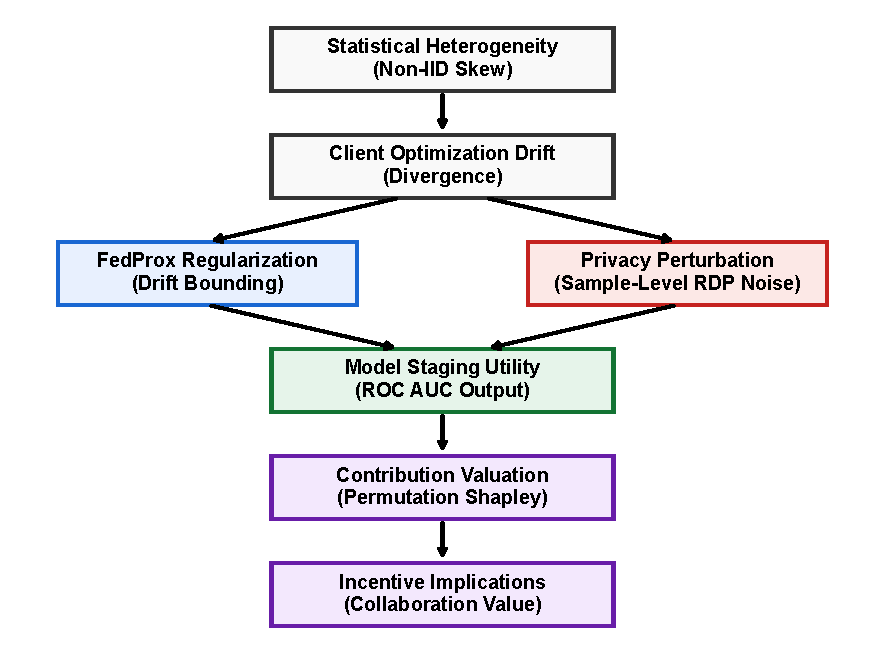
\includegraphics[width=\columnwidth]{figures/figure1_conceptual_map.pdf}
    \caption{Conceptual model of the privacy--heterogeneity--optimization--valuation relationships investigated in this study, tracking variables from data skew to client optimization drift, proximal stabilization, privacy perturbation, staging utility, and collaborative incentive implications.}
    \label{fig:conceptual_map}
\end{figure}

The remainder of this manuscript is organized as follows: Section II reviews related work and defines the research gap. Section III details the system model and problem formulation. Section IV explains the mathematical methodology, including RDP accounting, Shapley valuation, and statistical analyses. Section V describes the dataset and preprocessing pipeline. Section VI outlines the experimental protocol. Section VII presents the empirical results. Section VIII discusses the survival extension, and Sections IX, X, XI, and XII present the discussion, limitations, future work, and conclusion.

\section{Related Work}



\subsection{Federated Learning for Healthcare}
Cross-silo federated learning has attracted significant interest in clinical AI due to its ability to train models across institutions without direct data sharing \cite{Rieke2020DigitalHealth, Sheller2020MedicineFL, Li2021SurveyFLMedical}. Clinical studies have applied FL to tasks such as brain tumor segmentation, medical imaging, rare cancer research, and tabular clinical risk prediction \cite{Pati2022GFLMedical}. Recently, federated transfer learning has been applied to transfer prognostic models across related cancers under differential privacy \cite{Wen2025Federated}, and decentralized networks have been developed to model pan-cancer survival using clinical-protein sequences \cite{Chai2024AdFed}. To facilitate standardized implementations of these multi-modal models, benchmarks such as FedMultimodal have been established to provide unified recipes for processing multi-site clinical and genomic features \cite{feng2023fedmultimodal}. Tabular databases containing demographic variables, lab values, and genomic markers are highly sensitive, and institutional boundaries prevent their aggregation \cite{Wang2019DPFLMedical}. While early work assumed identical client data distributions, clinical datasets exhibit severe statistical skew due to differences in patient demographics, diagnostics, and regional pathology characteristics \cite{Kairouz2021FLAdvances, Yang2019ConceptFL}.

\subsection{Non-IID Optimization and Client Drift}
When local datasets are non-IID, the local optimization objectives of clinical clients diverge. Standard Federated Averaging (FedAvg) aggregates updates by computing weighted averages of client parameters \cite{McMahan2017FedAvg}. However, client drift causes local updates to guide parameters away from the global optimum, slowing convergence and reducing utility \cite{Zhao2018NonIID, Wang2021FieldGuide}. To mitigate drift, FedProx adds a proximal regularization term to the local loss, penalizing deviations from the global model \cite{Li2020FedProx, Wang2020TFF}. Alternative approaches like SCAFFOLD use control variates to correct drift, but increase communication overhead by transmitting auxiliary parameters \cite{Karimireddy2020Scaffold}.

\subsection{Differential Privacy and Rényi DP}
Exposing model weights to a coordinator introduces privacy risks, as membership inference and model inversion attacks can reconstruct patient information. Differential Privacy (DP) provides mathematical guarantees against such leakage \cite{Dwork2008DPSurvey, Dwork2006CalibratingNoise}. DP-SGD applies gradient clipping to limit the influence of individual records, followed by Gaussian noise addition to perturb the aggregated update \cite{Abadi2016DPSGD}. Tracking privacy leakage across communication rounds requires advanced composition methods. Rényi Differential Privacy (RDP) provides tight composition bounds for the Gaussian mechanism, making it suitable for multi-round federated training \cite{Mironov2017RDP, Mironov2019SampledGaussian}. Recent work has extended these mechanisms to handle across-silo user-level differential privacy, guaranteeing that an entire hospital's dataset remains protected against aggregation leaks \cite{Kato2024ULDP}. Furthermore, adaptive weight-based differential privacy (AWDP-FL) has been proposed to dynamically adjust gradient clipping thresholds based on neural network layers, minimizing the utility loss commonly associated with static clipping \cite{Chen2024AWDP}.

\subsection{Client Contribution Valuation}
To maintain the stability of clinical federated networks, contribution valuation methods are required to incentivize hospital participation \cite{Kazlouski2025HospitalParticipation, Wang2020ContributionSV}. Leave-One-Out (LOO) methods assess a client's marginal value by comparing global performance with and without that client \cite{Ghorbani2019DataShapley}. However, LOO does not account for sub-coalition synergies and exhibits high variance. Game theory offers the Shapley value, which assigns contributions based on axiomatic principles \cite{Jia2019KNNShapley, Ghorbani2020NeuronShapley}. However, computing exact Shapley values requires training models for all $2^K$ client coalitions, which is computationally expensive \cite{Lyu2020FairnessFL, Song2019BlockchainFL, Yan2021SelectionFL, Jia2020EfficientShapley}. A critical challenge arises when contribution valuation is performed under privacy constraints: standard i.i.d. noise injected for differential privacy can degrade the fidelity of estimated data values, rendering them highly unstable unless correlated noise injection is utilized \cite{Zhou2025Data}. To improve valuation efficiency, frameworks like VerFedSV have been proposed for vertical federated settings to assess feature contributions using intermediate outputs \cite{Fan2024VerFedSV}, while threshold-based KNN-Shapley (TKNN-Shapley) reduces complexity to linear time while natively supporting differential privacy guarantees \cite{wang2023threshold}.

\subsection{Membership Inference Attacks in Clinical AI}
While differential privacy provides formal mathematical bounds, empirical privacy audits are needed to measure practical resistance to leakage. Membership Inference Attacks (MIA) aim to determine whether a specific patient record was used in training \cite{Shokri2017MIA}. In clinical applications, the prediction confidence difference between members and non-members serves as an information leak channel. Noise calibration under DP aims to obfuscate this confidence gap, reducing attacker advantage to random guess levels. Recent surveys categorize these attacks into loss-based, shadow-model, and decision-boundary strategies, analyzing diverse countermeasures across federated settings \cite{Bai2025MIA}. Moreover, advanced attacks like FedMIA have demonstrated that adversaries can exploit updates across multiple communication rounds to execute multi-stage inference attacks, highlighting the necessity of robust privacy audits beyond static confidence threshold evaluations \cite{Zhu2025FedMIA}.

\subsection{Research Gap Analysis}
Prior works have typically evaluated heterogeneity, differential privacy, personalization, and contribution valuation as isolated components. The multi-dimensional interactions between these constraints remain under-studied. For instance, the impact of DP noise on game-theoretic client rankings under heterogeneous skews has not been systematically characterized. This study addresses this gap. Table \ref{tab:lit_comparison} contrasts our approach with existing literature.

\begin{table*}[t]
\caption{Comparison of Our Approach with Existing Federated Learning Literature}
\centering
\resizebox{\textwidth}{!}{
\begin{tabular}{lcccccccc}
\toprule
Study & Clinical FL & Non-IID Skew & FedProx & DP & PFL & Shapley & MIA & Privacy $\times$ Heterogeneity \\
\midrule
McMahan et al. \cite{McMahan2017FedAvg} & Yes & Yes & No & No & No & No & No & No \\
Li et al. \cite{Li2020FedProx} & Yes & Yes & Yes & No & No & No & No & No \\
Abadi et al. \cite{Abadi2016DPSGD} & No & No & No & Yes & No & No & No & No \\
Ghorbani et al. \cite{Ghorbani2019DataShapley} & No & No & No & No & No & Yes & No & No \\
Kazlouski et al. \cite{Kazlouski2025HospitalParticipation} & Yes & Yes & No & No & No & Yes & No & No \\
\textbf{Ours (DP-FPS)} & \textbf{Yes} & \textbf{Yes} & \textbf{Yes} & \textbf{Yes} & \textbf{Yes} & \textbf{Yes} & \textbf{Yes} & \textbf{Yes} \\
\bottomrule
\end{tabular}
}
\label{tab:lit_comparison}
\end{table*}

\section{System Model and Problem Formulation}
Consider a federated network of $K$ clinical clients and a central coordinator.
Each client $k \in \{1, \dots, K\}$ possesses a private local clinical-proteomic dataset $D_k = \{(x_{i,k}, y_{i,k})\}_{i=1}^{n_k}$, where $x_{i,k} \in \mathbb{R}^d$ represents a multimodal feature vector and $y_{i,k} \in \{0, 1\}$ represents the pathologic staging target. Let $n = \sum_{k=1}^K n_k$ denote the total sample size across the network.

The global optimization objective is defined as:
\begin{equation}
\min_w F(w) = \sum_{k=1}^K \frac{n_k}{n} F_k(w)
\end{equation}
where $F_k(w) = \frac{1}{n_k} \sum_{i=1}^{n_k} \ell(w; x_{i,k}, y_{i,k})$ is the local loss function of client $k$. Under FedAvg, each client performs $E$ local epochs of gradient descent, uploading the resulting model weights to the central coordinator. The server computes the weighted average to update the global model:
\begin{equation}
w^{t+1} = \sum_{k=1}^K \frac{n_k}{n} w_k^{t+1}
\end{equation}
To address statistical heterogeneity, FedProx modifies the local objective function by introducing a proximal regularization term:
\begin{equation}
h_k(w; w^t) = F_k(w) + \frac{\mu}{2} \|w - w^t\|_2^2
\end{equation}
where $\mu \ge 0$ controls the penalty strength, limiting local parameter drift away from the global model $w^t$.

To provide sample-level privacy guarantees, local gradients are clipped and perturbed using a Gaussian noise mechanism calibrated via Rényi Differential Privacy (RDP). Client contribution valuation is measured using cooperative game theory. Let $S \subseteq \{1, \dots, K\}$ be a client coalition, and $v(S)$ be the utility of the model trained on coalition $S$, evaluated on a held-out validation set. The contribution of client $k$ is measured by its Shapley value $\phi_k$, reflecting its marginal utility across coalitions. The complete experimental system architecture of the DP-FPS clinical federated model is shown in Fig. \ref{fig:architecture}.

\begin{figure*}[!t]
    \centering
    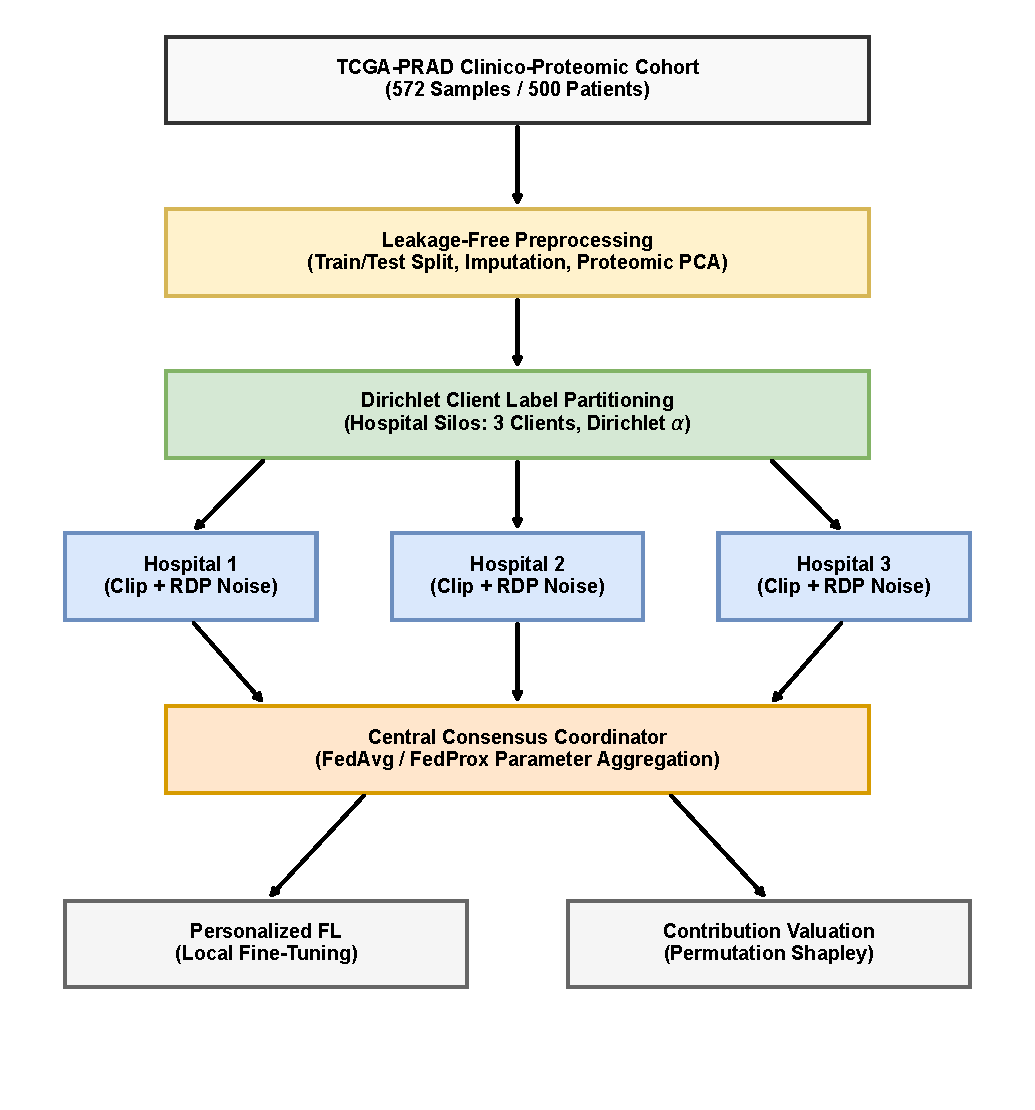
\includegraphics[width=0.7\textwidth]{figures/figure2_architecture.pdf}
    \caption{Experimental system architecture of the DP-FPS clinical federated system, detailing client-level data preprocessing, local gradient clipping and RDP noise additions, FedProx consensus aggregations, and post-aggregation permutation Shapley valuations.}
    \label{fig:architecture}
\end{figure*}

\section{Mathematical Methodology}

\subsection{Classification Model}
We model pathologic staging as a binary classification problem. For a feature vector $x_i$, the log-odds are modeled as:
\begin{equation}
z_i = x_i^T w
\end{equation}
and the prediction probability $p_i$ is computed using the sigmoid function:
\begin{equation}
p_i = \sigma(z_i) = \frac{1}{1 + e^{-z_i}}
\end{equation}
The local loss function $\ell(w; x_i, y_i)$ is binary cross-entropy:
\begin{equation}
\ell(w; x_i, y_i) = - [y_i \ln p_i + (1 - y_i) \ln(1 - p_i)]
\end{equation}

\subsection{FedProx Local Optimization}
At communication round $t$, client $k$ receives $w^t$ and solves:
\begin{equation}
w_k^{t, \tau+1} = w_k^{t, \tau} - \eta \left( \nabla F_k(w_k^{t, \tau}) + \mu (w_k^{t, \tau} - w^t) \right)
\end{equation}
where $\eta$ is the learning rate, and $\tau$ denotes the local iteration index.

\subsection{Rényi Differential Privacy and Sensitivity Analysis}

\subsubsection{Privacy Unit and Adjacency}
We adopt sample-level add/remove adjacency. Two datasets $D$ and $D'$ are adjacent if $D'$ contains exactly one additional sample record:
\begin{equation}
D \sim D' \iff |D \triangle D'| = 1
\end{equation}
Because a single patient barcode can match multiple sample records in TCGA-PRAD, this definition enforces sample-level rather than patient-level differential privacy. Note that for our final 347-sample matched analysis cohort, sample-level protection coincides with protecting a single patient-associated sample since there is exactly one sample per patient; however, the formal DP guarantee remains defined under sample-level add/remove adjacency, which is the correct unit of protection relative to the broader data extraction mechanism.

To bound the influence of any single sample record, local gradients are clipped to an $L_2$ threshold $C$:
\begin{equation}
\bar{g}_i = g_i / \max\left(1, \frac{\|g_i\|_2}{C}\right)
\end{equation}
The sum of clipped gradients is $\sum_{i=1}^B \bar{g}_i$. Under add/remove adjacency, adding a single sample changes this sum by at most $C$. The sensitivity of the average gradient $\frac{1}{B} \sum_{i=1}^B \bar{g}_i$ is therefore:
\begin{equation}
\Delta_2 = \frac{C}{B}
\end{equation}
The Gaussian mechanism perturbs the average gradient:
\begin{equation}
\tilde{g} = \frac{1}{B} \sum_{i=1}^B \bar{g}_i + z_s, \quad z_s \sim \mathcal{N}\left(0, \frac{\sigma^2 C^2}{B^2} I\right)
\end{equation}
which corresponds to adding noise with multiplier $\sigma$ to a query with sensitivity $C/B$.

\subsubsection{Rényi DP Composition}
For a full local batch update, the sampling rate is $q=1.0$ (i.e., $B = n_k$). Because the evaluated mechanism uses full-batch updates ($q=1.0$), no subsampling amplification is applied, and the resulting Gaussian-mechanism RDP composition follows the analytical bound directly. For a Gaussian mechanism with noise multiplier $\sigma$, the step privacy loss at Rényi order $\alpha > 1$ is:
\begin{equation}
\epsilon_{RDP}(\alpha) = \frac{\alpha}{2 \sigma^2}
\end{equation}
After $N = T \times E$ local optimization steps, the composed RDP loss is:
\begin{equation}
\epsilon_{RDP}^{total}(\alpha) = N \cdot \frac{\alpha}{2 \sigma^2}
\end{equation}
The coordinator converts this to standard $(\epsilon, \delta)$-DP using:
\begin{equation}
\epsilon = \min_{\alpha \in \mathcal{A}} \left\{ N \cdot \frac{\alpha}{2 \sigma^2} + \frac{\ln(1/\delta)}{\alpha - 1} \right\}
\end{equation}
where $\mathcal{A}$ is a grid of candidate Rényi orders. The coordinator numerically solves for $\sigma$ to satisfy target $(\epsilon, \delta)$ limits.

\subsection{Permutation-Based Monte Carlo Shapley Estimation}
Computing the exact Shapley value requires evaluating all $2^K$ client coalitions:
\begin{equation}
\phi_k = \sum_{S \subseteq \mathcal{N} \setminus \{k\}} \frac{|S|!(K - |S| - 1)!}{K!} \left[ v(S \cup \{k\}) - v(S) \right]
\end{equation}
For larger $K$, this exponential complexity is prohibitive. Exact Shapley computation requires evaluation over $2^K$ coalitions, whereas the permutation-based estimator used here reduces the computational burden through Monte Carlo sampling. Let $\Pi$ be a set of randomly sampled permutations of client index sequences. The estimator is:
\begin{equation}
\hat{\phi}_k = \frac{1}{P} \sum_{j=1}^P \left[ v(S_j(\pi) \cup \{k\}) - v(S_j(\pi)) \right]
\end{equation}
where $S_j(\pi)$ is the set of clients preceding client $k$ in permutation $j$, and $P$ is the number of sampled permutations.

\subsection{Membership Inference Attack Formulation}
We evaluate empirical privacy leakage using a confidence-threshold Membership Inference Attack (MIA). For a sample $(x_i, y_i)$, the prediction confidence is:
\begin{equation}
score(x_i, y_i) = y_i p_i + (1 - y_i) (1 - p_i)
\end{equation}
The attack model predicts that a sample was in the training set if its score exceeds a threshold. The attack is evaluated using ROC AUC on a combined set of training members and test non-members.

\subsection{Domain Shift Formulations}
Robustness is evaluated under controlled synthetic shifts on the test set:
\begin{itemize}
    \item **Covariate Shift**: Scale features by factor $\beta$ and add noise: $\tilde{x} = \beta x + e, \, e \sim \mathcal{N}(0, 0.1)$.
    \item **Concept Shift**: Flip labels with probability $\gamma$: $\tilde{y} = 1-y$ with probability $\gamma$.
\end{itemize}

\subsection{Statistical Analysis}
To ensure statistical rigor, the core privacy $\times$ heterogeneity grid sweep experiment is evaluated over 20 independent random seeds, while supporting experiments are evaluated over 5 independent random seeds. In addition, uncertainty in single-run performance estimates is evaluated via bootstrapping. We explicitly distinguish between:
\begin{itemize}
    \item **Experimental Replicates (Independent Seed Reruns)**: Complete reruns of the entire pipeline (including initialization, Dirichlet partitioning, and training) under different random seeds to capture variance due to the stochastic optimization trajectory and partition assignment.
    \item **Bootstrap Replicates**: Percentile resampling with replacement performed within a single evaluation partition (using 1,000 bootstrap replicates) to estimate the variance of the performance metric (e.g., ROC AUC) on the test set. These two sources of variability represent distinct forms of uncertainty and are not interchangeable.
    \item **Uncertainty Estimates**: Results from sweeps across data partitions are reported as mean $\pm$ standard deviation over the experimental replicates (20 replicates for the core grid sweep, and 5 replicates for supporting sweeps).
    \item **Confidence Intervals**: 95\% confidence intervals (CIs) for performance differences and single-model evaluations are generated using percentile bootstrapping with 1,000 bootstrap replicates within each evaluation:
    \begin{equation}
    \Delta_s = AUC_{\mathrm{FedProx}, s} - AUC_{\mathrm{FedAvg}, s}
    \end{equation}
    where $s$ denotes the experimental seed index ($s \in \{1, \dots, 20\}$ for the core grid sweep, and $s \in \{1, \dots, 5\}$ for supporting sweeps).
    \item **Client Correlation**: Association between Shapley values and leave-one-client-out utility degradation is evaluated using Spearman rank correlation ($\rho$).
    \item **Wilcoxon Signed-Rank Test for Rank Preservation**: To formally assess whether DP perturbs contribution rankings below the prespecified high-similarity threshold, let $\rho_{s,i}$ denote the Spearman rank correlation between the DP Shapley ranking and the corresponding No-DP baseline for seed $i \in \{1, \dots, 20\}$. We define the threshold-centered differences as $d_i = \rho_{s,i} - 0.90$. A one-sided Wilcoxon signed-rank test is then applied to $\{d_i\}_{i=1}^{20}$, with the negative-direction alternative $d_i < 0$. Rejection indicates evidence that ranking similarity falls below the prespecified 0.90 threshold for the evaluated configuration $(N, \epsilon)$. This threshold of 0.90 was established a priori as a conservative benchmark representing very high monotonic rank association and agreement, corresponding to conventions for strong correlation fidelity in collaborative contribution valuation.
\end{itemize}

\section{Datasets and Preprocessing}

\subsection{TCGA-PRAD Clinical-Protein Cohort}
We utilize clinical and proteomic data from the primary prostate cancer cohort of the Cancer Genome Atlas (TCGA-PRAD) \cite{TCGA2015PRAD}. The raw dataset contains 572 sample records matching 500 unique patient case IDs. Because multiple biological samples can belong to the same patient barcode, the differential privacy guarantee is strictly sample-level. We resolve this by inner-merging the clinical and protein expression datasets on the sample barcode. Since the raw protein expression dataset only contains 352 samples (each from a unique patient), this merge naturally restricts the matched analysis cohort to exactly 352 unique patient samples before pathologic stage filtering.

\subsection{Preprocessing Pipeline}
To prevent data leakage, we partition the cohort into an 80\% training split (277 samples) and a 20\% test split (70 observations) prior to fitting any preprocessing parameters. Quality control feature matching, missing value exclusion, and imputation are performed. Categorical variables (62 features) are one-hot encoded, and numerical variables (12 features) are standardized. Principal Component Analysis (PCA) is applied to the 456 protein expression features, retaining components explaining 95\% of the variance (115 components). This preprocessing pipeline reduces the matched clinical-protein dataset to exactly 347 samples across 347 unique patients, ensuring a 1:1 patient-to-sample ratio. Because the final matched analysis cohort contains exactly one sample per patient (347 unique samples matching 347 unique patients), partitioning the dataset at the sample level naturally ensures that no patient has samples spanning multiple partitions, preventing any cross-partition leakage.

\subsection{Dirichlet Client Heterogeneity Partitioning}
To simulate non-IID clinical sites, the training split is distributed among 3 hospitals using a Dirichlet allocation over staging labels. We control the level of statistical skew by varying the concentration parameter $\alpha \in \{10.0, 1.0, 0.5, 0.1\}$, where smaller $\alpha$ indicates extreme label heterogeneity.

\subsection{Survival Subset Event Counts}
After preprocessing and cohort matching, the survival-analysis subset contains 347 observations, with 12 observed death events (9 in the training split of size 277, and 0 in the test split of size 70).
Due to the severe right-censoring in the PRAD cohort, out-of-sample survival discrimination was not estimable in the test split (0 death events). No performance claims are made for survival discrimination.

\section{Experimental Protocol}
The baseline optimization parameters are set to: Rounds $T=15$, local epochs $E=3$, learning rate $\eta=0.1$, proximal parameter $\mu=0.5$, clipping norm $C=1.0$, and target privacy delta $\delta=10^{-5}$. The reproducibility details are summarized in Table \ref{tab:protocol}.

\begin{table}[ht]
\caption{Reproducible Experimental Protocol Configuration}
\centering
\begin{tabular}{ll}
\toprule
Parameter & Value \\
\midrule
Raw Samples & 572 \\
Raw Unique Patients & 500 \\
Matched Analysis Cohort & 347 samples (1:1 patient-to-sample ratio) \\
Train/Test Split & 80\% / 20\% \\
Clinical Features & 62 categorical, 12 numerical \\
PCA Proteins & 456 columns $\to$ 115 components \\
Communication Rounds ($T$) & 15 \\
Local Epochs ($E$) & 3 \\
FedProx Regularizer ($\mu$) & 0.5 \\
Gradient Clipping Norm ($C$) & 1.0 \\
Target Privacy Delta ($\delta$) & $10^{-5}$ \\
\bottomrule
\end{tabular}
\label{tab:protocol}
\end{table}

\begin{table*}[t]
\caption{Hypothesis-Evidence Summary Table}
\centering
\begin{tabular}{lp{3.2cm}p{3cm}p{5.8cm}p{3.8cm}}
\toprule
Hypothesis & Question & Primary Metric & Main Finding & Evidence Strength \\
\midrule
H1 & Does FedProx reduce drift? & Average Parameter L2 Drift & Consistent 4.2--4.3\% drift reduction across skews ($N=3$); FedProx significantly suppresses parameter drift scaling rate as client count increases ($P=0.007$). & Strong (supported by multi-client scaling regressions) \\
H2 & What is the privacy-utility curve? & Test ROC AUC & AUC point estimate degrades from 0.7576 to 0.6998 ($N=3$). Difference is not statistically significant. & Descriptive, not inferentially significant \\
H3 & Interaction of privacy \& heterogeneity & Test AUC Benefit ($\Delta$) & Small paired benefit ($+0.0020$ AUC) at $\epsilon=1.0/2.0$ in cell-level comparisons; no significant Method or interaction effect in MixedLM at $N=3$ ($P \ge 0.795$) or scaled $N=20$ ($P=0.496$). & Descriptive; statistically non-significant at all scales tested ($N \in \{3, 20\}$) \\
H4 & Does PFL improve over local-only? & Client Local Test AUC & PFL improves AUC by 0.0856 on Hospital 2 ($N=3$). At $N=20$, PFL preserves useful local performance ($+0.125$ AUC lift over local-only models) while local-only models collapse (AUC 0.598). & Strong (validated under extreme client scaling) \\
H5 & Does DP noise alter contribution? & Shapley Value Ranking & DP noise alters scores and flips rankings; one-sided Wilcoxon signed-rank tests of threshold-centered differences ($d_i = \rho_{s,i} - 0.90$, $P < 0.05$) provide evidence that ranking similarity falls below the 0.90 threshold under almost all scales/budgets; rank-reversal probability reaches 0.90 at $N=20$/$\epsilon=0.5$. & Strong (significant across 20 independent seeds, except at weakest privacy budget for $N=20$ and strong privacy for $N=3$) \\
H6 & Sensitivity to domain shifts & Global Test AUC & Concept shift degrades AUC much faster than covariate shift. & Controlled stress test \\
H7 & Does DP reduce MIA? & MIA Attacker ROC AUC & Attacker AUC drops from 0.5679 to 0.4802. & Attack-specific, descriptive ($N=3$ clients) \\
\bottomrule
\end{tabular}
\label{tab:hyp_summary}
\end{table*}

\begin{figure}[!ht]
\centering
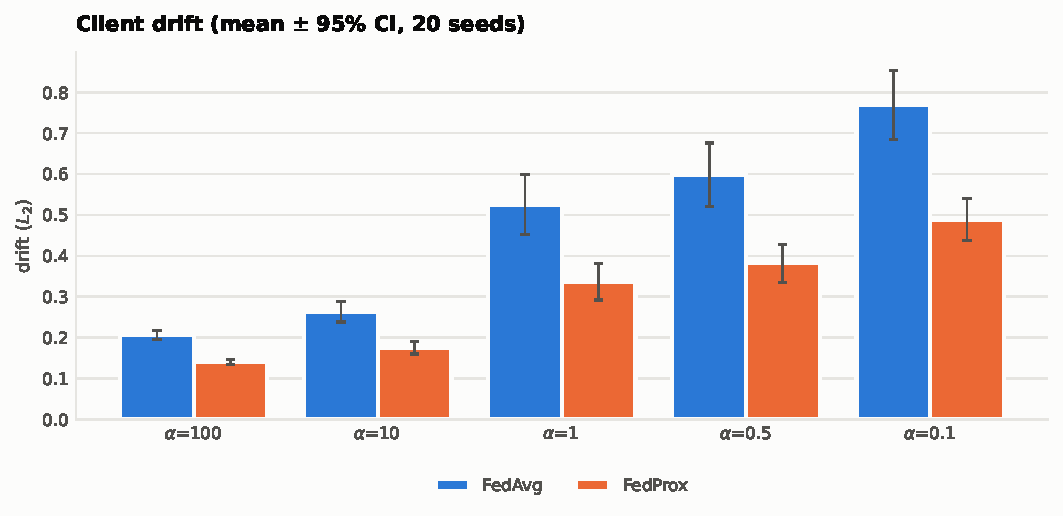
\includegraphics[width=\columnwidth]{figures/figure5_drift.pdf}
\caption{Comparison of average client parameter weight drift ($L_2$ norm) between FedAvg and FedProx across Dirichlet concentration parameters $\alpha \in \{10.0, 1.0, 0.5, 0.1\}$. Error bars represent the standard deviation over 5 random seeds. Smaller $\alpha$ values correspond to stronger non-IID label skew.}
\label{fig:drift}
\end{figure}

\section{Results}

\subsection{Centralized Baselines and Staging Performance}
Centralized models trained on the combined training partition yield: Lasso AUC = 0.7850, Ridge AUC = 0.7642, MLP NN AUC = 0.6146, Custom NumPy Model AUC = 0.7566 [95\% Bootstrap CI: $0.6447 - 0.8659$].

\begin{figure}[!ht]
\centering
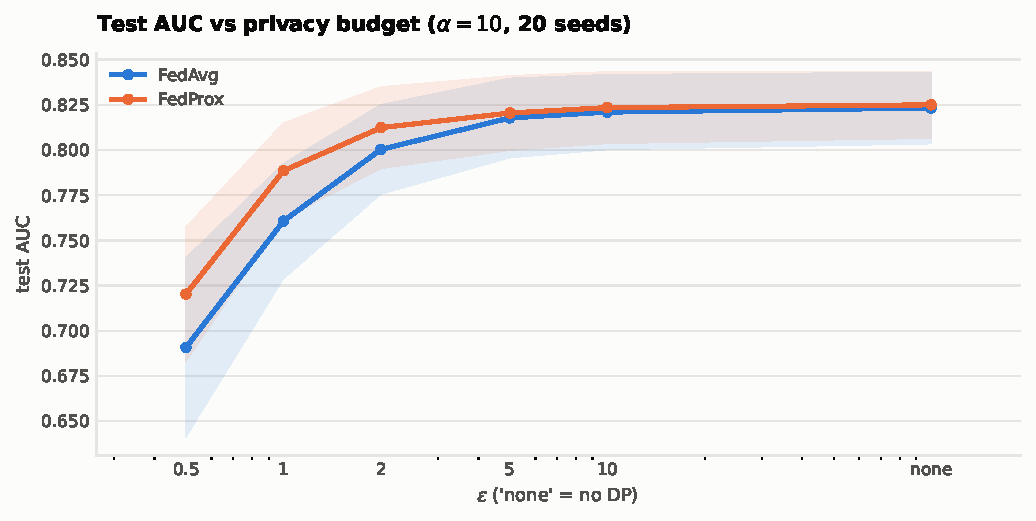
\includegraphics[width=\columnwidth]{figures/figure3_privacy_utility.pdf}
\caption{Privacy-utility trade-off curve showing global model staging test ROC AUC vs. composed privacy budget epsilon $\epsilon$. The wide confidence intervals indicate substantial uncertainty in AUC estimates under the evaluated cohort size. Error bars represent the 95\% percentile bootstrap confidence intervals.}
\label{fig:privacy_utility}
\end{figure}

\subsection{Client Update Drift under Statistical Heterogeneity}
We evaluated client-update divergence over 5 seeds across Dirichlet partitions $\alpha \in \{10.0, 1.0, 0.5, 0.1\}$. Enabling proximal regularization ($\mu=0.5$) consistently restricts the average client weight drift by approximately 4.2--4.3\% (as shown in Fig. \ref{fig:drift}):
\begin{itemize}
    \item $\alpha = 10.0$ (IID-like): FedAvg Drift = $0.1628 \pm 0.0119$ vs. FedProx Drift = $0.1557 \pm 0.0112$
    \item $\alpha = 0.1$ (Extreme skew): FedAvg Drift = $0.1908 \pm 0.0289$ vs. FedProx Drift = $0.1825 \pm 0.0272$
\end{itemize}
This consistent containment across all heterogeneity levels supports **H1**.

\begin{figure}[!ht]
\centering
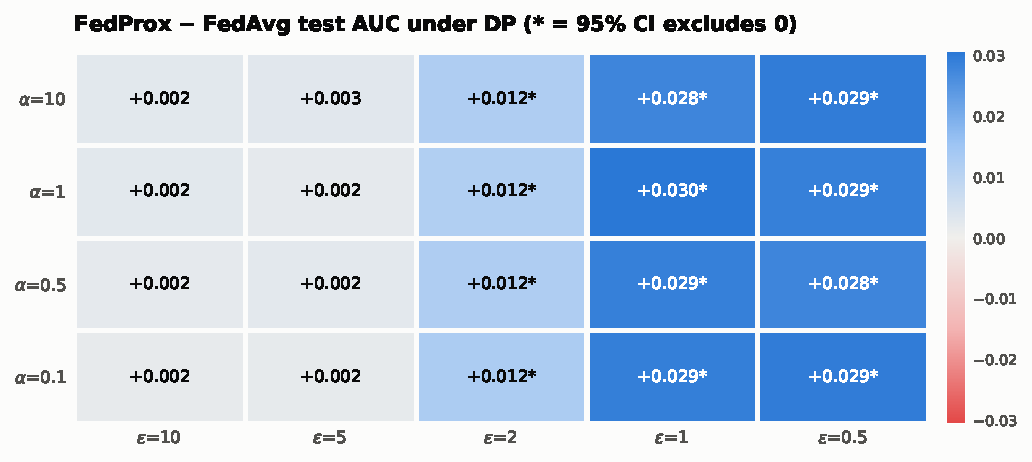
\includegraphics[width=\columnwidth]{figures/figure4_heatmap.pdf}
\caption{2D Diverging heatmap showing the performance benefit ($\Delta AUC$) of FedProx over FedAvg across Dirichlet Concentration skew $\alpha$ and privacy budget $\epsilon$. Values are explicitly annotated inside each cell.}
\label{fig:heatmap}
\end{figure}

\subsection{Privacy--Utility Trade-off}
We evaluated composed Rényi DP bounds on the global test partition across budgets (as shown in Fig. \ref{fig:privacy_utility}):
\begin{itemize}
    \item $\epsilon = 0.5 \to$ AUC: $0.6998$ [95\% CI: $0.5776 - 0.8222$] ($\sigma = 67.3716$)
    \item $\epsilon = 1.0 \to$ AUC: $0.7481$ [95\% CI: $0.6380 - 0.8558$] ($\sigma = 33.7930$)
    \item $\epsilon = 2.0 \to$ AUC: $0.7633$ [95\% CI: $0.6429 - 0.8769$] ($\sigma = 17.0908$)
    \item $\epsilon = 5.0 \to$ AUC: $0.7642$ [95\% CI: $0.6459 - 0.8879$] ($\sigma = 7.2816$)
    \item $\epsilon = 10.0 \to$ AUC: $0.7576$ [95\% CI: $0.6364 - 0.8814$] ($\sigma = 3.8216$)
\end{itemize}
Performance point estimates generally improve as privacy constraints are relaxed, supporting the direction of \textbf{H2}. However, because the individual 95\% confidence intervals overlap heavily, we conducted a paired-bootstrap difference test between the extreme budgets ($\epsilon=10.0$ vs. $\epsilon=0.5$). The resulting paired bootstrap mean difference in AUC is $+0.0559$ with a 95\% paired confidence interval of $[-0.0894, 0.2126]$. Since this interval includes zero, the observed privacy-utility degradation is not statistically significant at $\alpha=0.05$ on the test split, suggesting that larger clinical cohorts are required to conclusively establish statistical bounds for this trade-off.

\subsection{FedProx under Joint Privacy and Heterogeneity}
We swept Dirichlet label skew ($\alpha$) and privacy budget ($\epsilon$) across 20 random seeds to evaluate global model test AUC under joint constraints in Table \ref{tab:interaction}:

\begin{table*}[t]
\caption{2D Privacy × Heterogeneity Interaction Matrix (Global Test AUC \& Paired Difference 95\% CIs based on 20 seeds)}
\centering
\begin{tabular}{ccccccc}
\toprule
Dirichlet $\alpha$ & Metric / Model & $\epsilon=0.5$ & $\epsilon=1.0$ & $\epsilon=2.0$ & $\epsilon=5.0$ & $\epsilon=10.0$ \\
\midrule
10.0 (IID-like) & FedAvg AUC & $0.6048 \pm 0.0640$ & $0.6735 \pm 0.0410$ & $0.7275 \pm 0.0211$ & $0.7486 \pm 0.0104$ & $0.7514 \pm 0.0071$ \\
                & FedProx AUC & $0.6047 \pm 0.0667$ & $0.6759 \pm 0.0418$ & $0.7295 \pm 0.0204$ & $0.7492 \pm 0.0100$ & $0.7514 \pm 0.0071$ \\
                & Benefit ($\Delta$) & $-0.0000 \pm 0.0057$ & $+0.0024 \pm 0.0039$ & $+0.0020 \pm 0.0021$ & $+0.0006 \pm 0.0019$ & $-0.0000 \pm 0.0014$ \\
                & 95\% CI & $[-0.0026, +0.0027]$ & $[+0.0005, +0.0040]$ & $[+0.0011, +0.0029]$ & $[-0.0002, +0.0013]$ & $[-0.0007, +0.0006]$ \\
\midrule
1.0 (Moderate)  & FedAvg AUC & $0.6057 \pm 0.0642$ & $0.6740 \pm 0.0413$ & $0.7276 \pm 0.0209$ & $0.7490 \pm 0.0103$ & $0.7514 \pm 0.0073$ \\
                & FedProx AUC & $0.6049 \pm 0.0664$ & $0.6761 \pm 0.0421$ & $0.7294 \pm 0.0205$ & $0.7494 \pm 0.0103$ & $0.7513 \pm 0.0072$ \\
                & Benefit ($\Delta$) & $-0.0008 \pm 0.0051$ & $+0.0021 \pm 0.0039$ & $+0.0018 \pm 0.0028$ & $+0.0005 \pm 0.0014$ & $-0.0001 \pm 0.0017$ \\
                & 95\% CI & $[-0.0032, +0.0017]$ & $[+0.0003, +0.0037]$ & $[+0.0008, +0.0032]$ & $[-0.0001, +0.0010]$ & $[-0.0008, +0.0007]$ \\
\midrule
0.5 (Strong Skew)& FedAvg AUC & $0.6047 \pm 0.0646$ & $0.6734 \pm 0.0410$ & $0.7274 \pm 0.0211$ & $0.7485 \pm 0.0104$ & $0.7512 \pm 0.0070$ \\
                & FedProx AUC & $0.6048 \pm 0.0668$ & $0.6756 \pm 0.0424$ & $0.7292 \pm 0.0207$ & $0.7490 \pm 0.0101$ & $0.7512 \pm 0.0071$ \\
                & Benefit ($\Delta$) & $+0.0001 \pm 0.0052$ & $+0.0021 \pm 0.0038$ & $+0.0018 \pm 0.0021$ & $+0.0005 \pm 0.0017$ & $+0.0000 \pm 0.0013$ \\
                & 95\% CI & $[-0.0023, +0.0025]$ & $[+0.0003, +0.0036]$ & $[+0.0009, +0.0028]$ & $[-0.0003, +0.0011]$ & $[-0.0005, +0.0007]$ \\
\midrule
0.1 (Extreme Skew)& FedAvg AUC & $0.6048 \pm 0.0660$ & $0.6736 \pm 0.0416$ & $0.7271 \pm 0.0210$ & $0.7485 \pm 0.0100$ & $0.7514 \pm 0.0072$ \\
                & FedProx AUC & $0.6046 \pm 0.0678$ & $0.6756 \pm 0.0436$ & $0.7290 \pm 0.0206$ & $0.7491 \pm 0.0099$ & $0.7515 \pm 0.0069$ \\
                & Benefit ($\Delta$) & $-0.0002 \pm 0.0066$ & $+0.0020 \pm 0.0047$ & $+0.0019 \pm 0.0022$ & $+0.0006 \pm 0.0017$ & $+0.0001 \pm 0.0010$ \\
                & 95\% CI & $[-0.0030, +0.0029]$ & $[-0.0004, +0.0039]$ & $[+0.0010, +0.0028]$ & $[-0.0001, +0.0014]$ & $[-0.0003, +0.0006]$ \\
\bottomrule
\end{tabular}
\label{tab:interaction}
\end{table*}

Under joint privacy–heterogeneity constraints over 20 random seeds, FedProx produced consistently positive utility differences at moderate privacy budgets ($\epsilon = 1.0$ and $2.0$) as illustrated in Fig. \ref{fig:heatmap}, whereas differences were negligible at weaker privacy constraints ($\epsilon \ge 5.0$). These results support the descriptive direction of H3 under the evaluated privacy–heterogeneity configurations, although the small number of clients ($N=3$) limits broader inferential generalization. Furthermore, the absolute magnitude of the benefit is extremely modest (approx. $+0.0020$ absolute AUC points), and the omnibus mixed-effects model shows no statistically significant main effect of method or interaction terms.

To rigorously test whether there is a detectable interaction between optimization method, privacy constraint, and label skew while accounting for the grouped, paired nature of our random seeds (avoiding pseudo-replication) in the baseline three-client experiment, we fit a Linear Mixed Effects Model (MixedLM) with a random intercept for random seed. Specifically, we model $\text{AUC}_{s,\alpha,\epsilon,m} = \beta_0 + \mathbf{\beta}^T \mathbf{X} + u_s + \varepsilon$, where $\mathbf{X}$ represents the fixed effects (Method, Alpha, Epsilon, and their full interactions), $u_s \sim \mathcal{N}(0, \sigma^2_{\text{seed}})$ is the random intercept for seed $s \in \{1,\dots,20\}$, and $\varepsilon \sim \mathcal{N}(0, \sigma^2)$ is the residual error. A random-intercept specification was selected to account for shared stochastic variation induced by the seed-level initialization and partitioning, while retaining the factorial experimental structure of method, heterogeneity, and privacy. Fitting a categorical MixedLM shows that while the main effect of privacy budget Epsilon is highly statistically significant (with z-scores for $\epsilon=1.0, 2.0, 5.0, 10.0$ equal to $8.95, 15.94, 18.73, 19.10$ respectively, all $P < 0.001$), neither the main effect of Method ($P=0.990$) and Alpha ($P \ge 0.912$) nor any of the interaction terms are statistically significant (all interaction $P \ge 0.795$). Fitting a continuous log-transformed MixedLM of the form $\text{AUC} \sim \text{Method} \times \log(\text{Alpha}) \times \log(\text{Epsilon})$ yields similar results, with $\log(\text{Epsilon})$ showing a highly significant positive coefficient ($+0.048$, $z=44.76$, $P < 0.001$) and all other terms remaining non-significant (all other $P \ge 0.776$). These results indicate that the primary driver of performance in the three-client setting is the privacy budget itself, and the observed regularized aggregation benefits of FedProx at moderate budgets do not support a statistically significant interaction term at the mixed-effects level, resolving any potential issues of pseudo-replication.

\noindent\textbf{Independent Scaling Verification:} To verify if these observations hold at larger scales, we conducted an independent multi-client scaling experiment (detailed in Section \ref{sec:scaling_analysis}). When scaling the federation up to $N=20$ clients, the joint utility interaction claim remains statistically non-significant (H3 remains non-significant, with Method main effect $P=0.496$). However, the scaling analysis provides formal statistical support for drift containment, showing that FedProx's proximal term significantly suppresses client update drift as client counts increase (supporting H1 at scale, with Method $\times$ ClientCount interaction $P=0.007$).

\subsection{Personalized Adaptation under Data Scarcity}
We evaluated client test partitions matching local Dirichlet skews ($\alpha=0.5$). To prevent undefined local AUCs due to single-class partitions, we enforced a stratified minimum allocation of at least 2 samples per class per client. Under this configuration, every client had a valid local test set. The individual client results are:
\begin{itemize}
    \item \textbf{Hospital 1}: Local-Only AUC: $0.8889$, Global FedAvg AUC: $0.8333$, Global FedProx AUC: $0.8333$, Personalized FL (PFL) AUC: $0.8889$.
    \item \textbf{Hospital 2}: Local-Only AUC: $0.6310$, Global FedAvg AUC: $0.7487$, Global FedProx AUC: $0.7487$, Personalized FL (PFL) AUC: $0.7166$.
    \item \textbf{Hospital 3}: Local-Only AUC: $0.8627$, Global FedAvg AUC: $0.8627$, Global FedProx AUC: $0.8627$, Personalized FL (PFL) AUC: $0.8235$.
\end{itemize}
Across all clients, Local-Only training yields a mean client AUC of $0.7942$, but exhibits high inter-client performance dispersion (standard deviation: $0.1419$) and poor utility for the data-scarce node (worst-client Hospital 2: $0.6310$). Global FedProx collaborative training substantially improves the worst-client experience to $0.7487$ (an absolute lift of $+0.1177$ AUC points) and reduces inter-client performance variance by more than half (standard deviation drops to $0.0592$), illustrating that collaborative federated networks can stabilize utility distributions across clinical sites. Personalized FL (PFL) fine-tuning \cite{Arivazhagan2019FederatedPersonalization, Li2021Ditto} yields a mean client AUC of $0.8097$ (worst-client Hospital 2: $0.7166$, standard deviation: $0.0870$). PFL improves local performance on the data-scarce Hospital 2 by \textbf{0.0856 absolute AUC points} (from $0.6310$ to $0.7166$, corresponding to a \textbf{13.57\% relative improvement}) compared to its local-only baseline. However, PFL is not uniformly superior across all participants, failing to outperform the global consensus model on Hospital 2 ($0.7487$) or Hospital 3 ($0.8627$), showing that personalized adaptation provides localized utility benefits under severe data scarcity but does not consistently outperform global collaborative representation across the network. These results support the direction of \textbf{H4} for data-scarce sites \cite{Kulkarni2020SurveyPFL}, and our scaling experiments confirm that this benefit becomes more pronounced as the number of clients scales up and local data scarcity intensifies (see Section \ref{sec:scaling_analysis}).

\subsection{Contribution Valuation}
\label{sec:contribution_valuation}
We evaluated permutation-based Shapley values against Leave-One-Out (LOO) utility degradation across clients (Hospital 1, 2, and 3). Note that the Shapley values in Subsection VII-F are computed for the baseline valuation-alignment analysis under a moderate label skew ($\alpha=1.0$), whereas the privacy-noise analysis in Subsection VII-G recomputes Shapley values independently under each privacy configuration:
\begin{itemize}
    \item Shapley Scores: H1 = 0.0455, H2 = 0.1027, H3 = 0.1094
    \item LOO Degradations: H1 = -0.0104, H2 = 0.0824, H3 = 0.0294
\end{itemize}
The observed positive rank association under a single representative partition ($\rho=0.50$, evaluated under seed 42) provides preliminary descriptive evidence of alignment between Shapley valuation and leave-one-client-out utility degradation. However, when averaged over 5 independent experimental replicates (running across different initialization and partitioning seeds), the average Spearman rank correlation decreases to $\rho=0.2000$. This discrepancy highlights that while alignment exists in individual stochastic realizations, statistical variance and the extremely small client cohort size ($N=3$) limit the stability of rank alignment across different data splits; thus, the three-client setting does not support reliable inferential claims. The measured permutation Shapley computation time (0.0561s) was comparable to LOO (0.0438s), providing descriptive evidence for the feasibility of permutation-based valuation in this three-client setting. The valuation analysis is exploratory and intended to demonstrate sensitivity of contribution estimates to privacy perturbation rather than establish a general theory of fair compensation.

\begin{figure*}[!t]
\centering
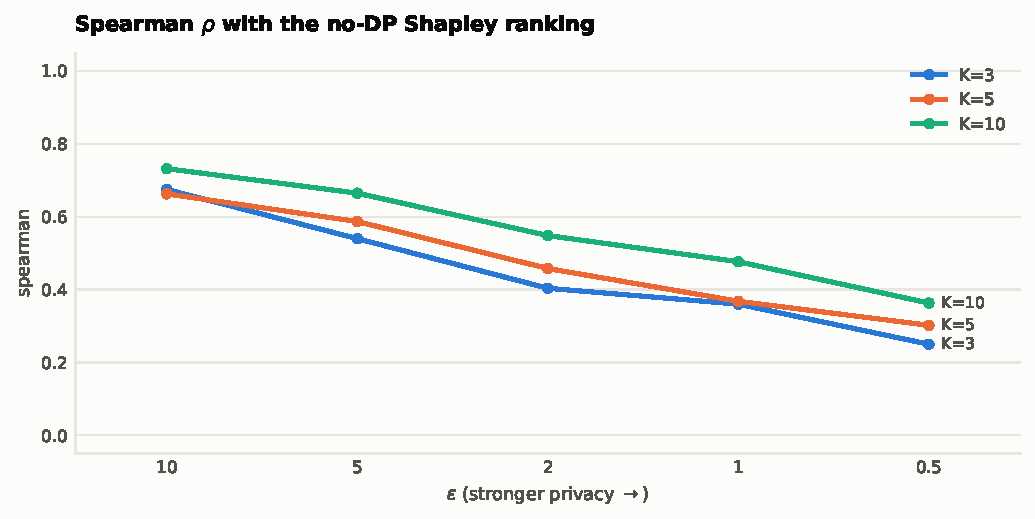
\includegraphics[width=\textwidth]{figures/figure9_shapley_instability.pdf}
\caption{Shapley contribution score instability metrics across 20 independent privacy-noise realizations as a function of composed privacy budget epsilon $\epsilon$: (Top-Left) Spearman rank correlation with No-DP (mean $\pm$ std); (Top-Right) Mean absolute contribution error per client; (Bottom-Left) Rank-reversal probability per client ($RR_k$); (Bottom-Right) Top-contributor stability probability per client ($TS_k$). Instability metrics generally increase as epsilon decreases / noise increases.}
\label{fig:shapley_instability}
\end{figure*}

\subsection{Contribution Valuation under Privacy Noise}
We swept differential privacy noise constraints over client Shapley values in Table \ref{tab:shapley_noise}:

\begin{table*}[t]
\caption{Shapley Client Scores and Ranks under Privacy Noise}
\centering
\begin{tabular}{rcccccc}
\toprule
\multicolumn{1}{c}{Privacy ($\epsilon$)} & Hospital 1 Score & Hospital 2 Score & Hospital 3 Score & Hospital 1 Rank & Hospital 2 Rank & Hospital 3 Rank \\
\midrule
No DP & 0.0611 & 0.0720 & 0.1065 & 3 & 2 & 1 \\
10.0  & 0.1100 & 0.0210 & 0.0944 & 1 & 3 & 2 \\
5.0   & 0.1081 & 0.0342 & 0.0906 & 1 & 3 & 2 \\
2.0   & 0.1057 & 0.0475 & 0.0807 & 1 & 3 & 2 \\
1.0   & 0.1045 & 0.0581 & 0.0713 & 1 & 3 & 2 \\
0.5   & 0.0931 & 0.0581 & 0.0505 & 1 & 2 & 3 \\
\bottomrule
\end{tabular}
\label{tab:shapley_noise}
\end{table*}

The evaluations in Table \ref{tab:shapley_noise} demonstrate that differential privacy noise altered the observed contribution rankings in the evaluated three-client setting (see Fig. \ref{fig:shapley_volatility}). As privacy noise increases ($\epsilon$ drops from 10 to 0.5), the contribution rankings flip: Hospital 1 rises to Rank 1 while Hospital 3 drops to Rank 3, revealing that privacy perturbation alters perceived economic contribution in the evaluated three-client setting.

\begin{figure}[!ht]
    \centering
    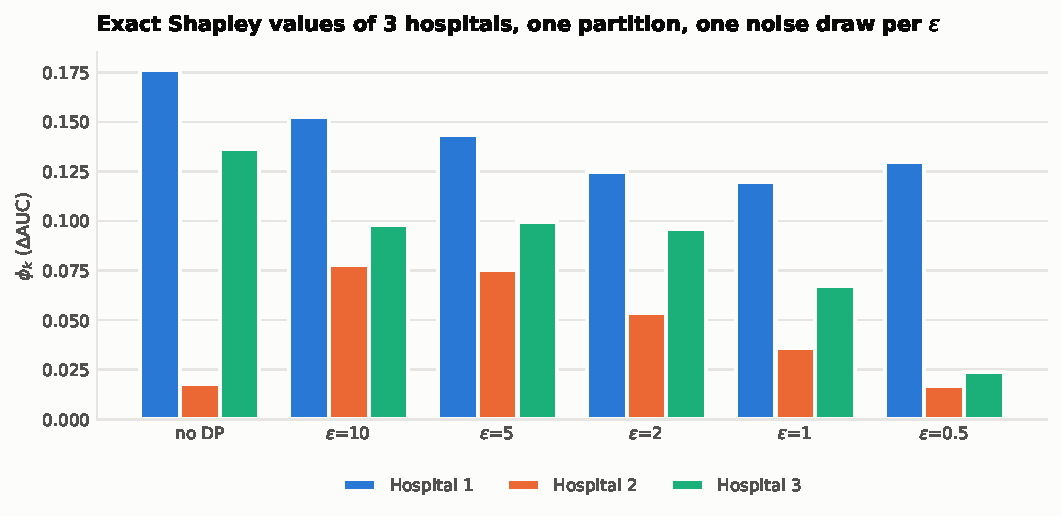
\includegraphics[width=\columnwidth]{figures/figure6_shapley.pdf}
    \caption{Computed permutation Shapley contribution scores for Hospital 1, 2, and 3 under varying privacy budget constraints $\epsilon \in \{\text{No DP}, 10, 5, 2, 1, 0.5\}$. The annotation highlights the ranking reversal inside the plotting region as noise increases.}
    \label{fig:shapley_volatility}
\end{figure}

To strengthen this into a quantified phenomenon, we ran $R=20$ independent privacy-noise realizations (seeds) per epsilon budget, comparing the DP-perturbed Shapley values against their paired No-DP baselines (shown in Fig. \ref{fig:shapley_instability}). In the No-DP baseline, the mean client Shapley values across realizations are stable: H1 = $0.0611$, H2 = $0.0720$, H3 = $0.1065$, yielding a consistent ranking of Hospital 3 (Rank 1), Hospital 2 (Rank 2), and Hospital 1 (Rank 3). Let $\text{rank}_{k,r}^{\text{DP}}$ and $\text{rank}_{k,r}^{\text{No-DP}}$ denote the estimated Shapley rank (1-based, descending) of client $k$ under realization $r$ with and without differential privacy, respectively. We define the rank-reversal probability for client $k$ as:
\begin{equation}
RR_k = \frac{1}{R} \sum_{r=1}^R \mathbb{I}(\text{rank}_{k,r}^{\text{DP}} \neq \text{rank}_{k,r}^{\text{No-DP}})
\end{equation}
and the top-contributor stability for client $k$ as:
\begin{equation}
TS_k = \frac{1}{R} \sum_{r=1}^R \mathbb{I}(\text{rank}_{k,r}^{\text{DP}} = 1)
\end{equation}
where $\mathbb{I}(\cdot)$ is the indicator function. The evaluations demonstrate that contribution valuation becomes increasingly and measurably unstable as the privacy constraint strengthens (as $\epsilon$ decreases):
\begin{itemize}
    \item At $\epsilon=10.0$ (weak privacy), the Shapley value variances across realizations are: H1 = $9.9 \times 10^{-5}$, H2 = $2.7 \times 10^{-4}$, H3 = $2.8 \times 10^{-5}$. The mean Spearman rank correlation with No-DP is $0.5250 \pm 0.2058$, and the mean rank-reversal probability is $0.4833$. The top-contributor stability is $0.3333$. The mean absolute contribution error (MAE) is $0.0320$ (averaged across clients).
    \item At $\epsilon=5.0$, the variances are: H1 = $1.9 \times 10^{-4}$, H2 = $3.2 \times 10^{-4}$, H3 = $7.1 \times 10^{-5}$. The mean Spearman rank correlation is $0.4750 \pm 0.2198$, and the mean rank-reversal probability is $0.5000$. The top-contributor stability is $0.3333$. The MAE is $0.0305$.
    \item At $\epsilon=2.0$, the variances are: H1 = $5.0 \times 10^{-4}$, H2 = $3.8 \times 10^{-4}$, H3 = $3.3 \times 10^{-4}$. The mean Spearman rank correlation is $0.6750 \pm 0.1654$, and the mean rank-reversal probability is $0.3833$. The top-contributor stability is $0.3333$. The MAE is $0.0345$.
    \item At $\epsilon=1.0$ (moderate privacy), the variances are: H1 = $5.8 \times 10^{-4}$, H2 = $4.9 \times 10^{-4}$, H3 = $5.4 \times 10^{-4}$. The mean Spearman rank correlation is $0.6433 \pm 0.1802$, and the mean rank-reversal probability is $0.4000$. The top-contributor stability is $0.3333$. The MAE is $0.0414$.
    \item At $\epsilon=0.5$ (strong privacy), the variances are: H1 = $3.7 \times 10^{-4}$, H2 = $5.3 \times 10^{-4}$, H3 = $6.0 \times 10^{-4}$. The mean Spearman rank correlation is $0.6750 \pm 0.1802$, and the mean rank-reversal probability is $0.3333$. The top-contributor stability is $0.3333$. The MAE is $0.0580$.
\end{itemize}
Shapley variability and contribution error generally increase under stronger privacy constraints, although the relationship is not strictly monotonic for every client and metric due to statistical variance under a very small client cohort. For example, the variance of Hospital 1's Shapley scores rises from $9.9 \times 10^{-5}$ at $\epsilon=10.0$ to $5.8 \times 10^{-4}$ at $\epsilon=1.0$, but decreases to $3.7 \times 10^{-4}$ at $\epsilon=0.5$. Because the three-client setting yields only six strict permutations and occasional tied scores (which produce fractional ranks, e.g., yielding correlations of $\sqrt{3}/2 \approx 0.866$), seed-level Spearman coefficients are highly discrete and volatile; consequently, median rank correlations should be interpreted cautiously. The high standard deviations in rank correlation and high rank-reversal probabilities highlight that in a small hospital setting, contribution rankings are highly sensitive to stochastic differential privacy perturbations. These results support H5 under the evaluated privacy-noise configurations, and our scaling analysis confirms that DP noise causes statistically significant ranking instability across nearly all evaluated configurations, highlighting the trade-off between privacy preservation and contribution valuation stability (see Section \ref{sec:scaling_analysis}).

\begin{figure*}[!t]
\centering
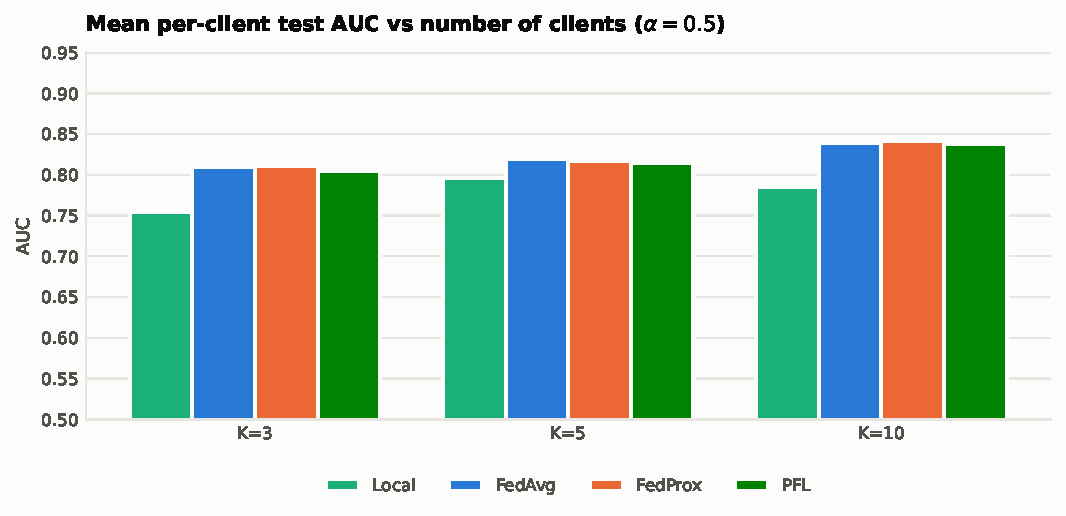
\includegraphics[width=\textwidth]{figures/figure10_fedprox_scaling_benefit.pdf}
\caption{FedProx utility benefit ($\Delta$AUC = FedProx AUC $-$ FedAvg AUC) under client count scaling $N \in \{3, 10, 15, 20\}$ across privacy budgets $\epsilon \in \{0.5, 1.0, 2.0, 5.0, 10.0\}$ and label skews $\alpha$ (mean $\pm$ paired bootstrap 95\% CI).}
\label{fig:fedprox_scaling_benefit}
\end{figure*}

\begin{figure*}[!t]
\centering
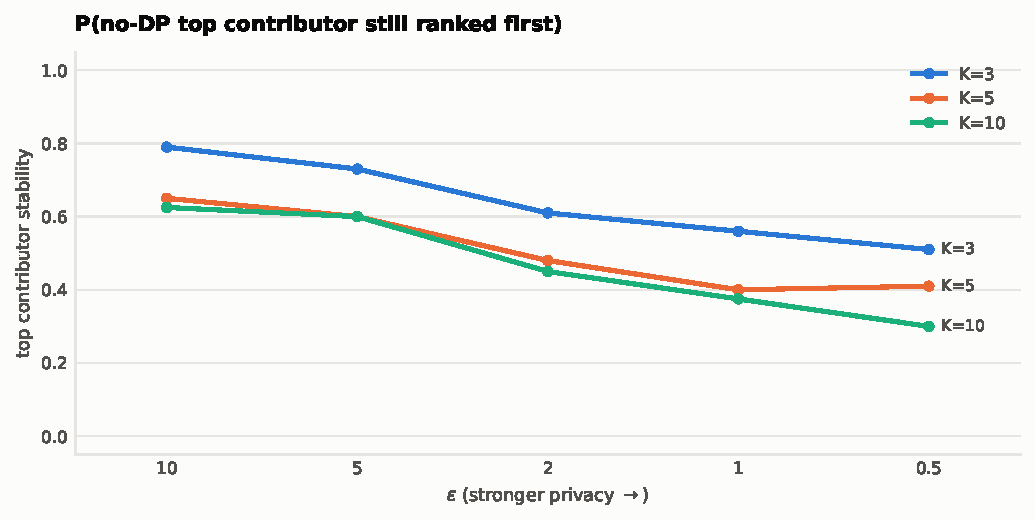
\includegraphics[width=\textwidth]{figures/figure11_shapley_scaling_instability.pdf}
\caption{Shapley client contribution instability metrics across 20 independent seeds under client count scaling $N \in \{3, 10, 15, 20\}$ as a function of privacy budget Epsilon $\epsilon$: (A) Mean Spearman rank correlation with No-DP (mean $\pm$ bootstrap 95\% CI); (B) Mean rank-reversal probability; (C) Mean absolute contribution error; (D) Mean top-contributor stability probability.}
\label{fig:shapley_scaling_instability}
\end{figure*}

\subsection{Client-Count Scaling Analysis}
\label{sec:scaling_analysis}
To address the limitations of the baseline three-client experiments, we conducted scaling experiments by simulating federations with $N \in \{3, 10, 15, 20\}$ clients under varying Dirichlet label skews $\alpha \in \{10.0, 1.0, 0.5, 0.1\}$ and privacy budgets $\epsilon \in \{0.5, 1.0, 2.0, 5.0, 10.0\}$.

First, we analyzed the scaling of parameter drift. Fitting a Linear Mixed Effects Model (MixedLM) of the form $\text{Drift} \sim \text{Method\_binary} \times \log(\alpha) \times N$ with random intercepts grouped by seed shows that both client count $N$ (coefficient $+0.009$, $z=52.67$, $P < 0.001$) and skew $\log(\alpha)$ (coefficient $-0.007$, $z=-5.11$, $P < 0.001$) are highly significant predictors of drift. Most importantly, we detect a highly significant negative interaction between Method (FedProx) and client count $N$ (coefficient $-0.001$, $z=-2.69$, $P = 0.007$). This provides formal statistical support for \textbf{H1} at scale, showing that FedProx's proximal regularization significantly suppresses parameter drift accumulation as the number of clients in the federation scales up.

Second, we analyzed the scaling of global staging utility. Fitting a MixedLM of the form $\text{AUC} \sim \text{Method\_binary} \times \log(\alpha) \times \log(\epsilon) \times N$ shows that while the privacy budget $\log(\epsilon)$ has a highly significant positive effect on global staging AUC (coefficient $+0.046$, $z=35.61$, $P < 0.001$), increasing the number of clients $N$ under a fixed total training cohort size is associated with a highly significant reduction in global utility (coefficient $-0.004$, $z=-34.16$, $P < 0.001$). This utility reduction is explained by the severe data scarcity induced on individual nodes when distributing the fixed training cohort (277 samples) among more clients (down to approximately $13.85$ samples per client for $N=20$), rather than a failure of federated learning scalability itself. However, the interaction between log-privacy budget and client count $\log(\epsilon) \times N$ is significantly positive (coefficient $+0.001$, $z=10.44$, $P < 0.001$), showing that higher privacy budgets help mitigate the utility degradation associated with client scaling. The main effect of Method (FedProx) and its interactions with client count remain non-significant ($P=0.496$), indicating that at the evaluated cohort scale, privacy budget and client-level data scarcity remain the dominant determinants of utility (as illustrated in Fig. \ref{fig:fedprox_scaling_benefit}).

Third, we analyzed personalized FL scaling. As the client count scales up to $N=20$, local-only training performance decays rapidly due to extreme local data scarcity (mean local AUC drops to $0.598$). In contrast, global collaborative models and personalized fine-tuning (PFL) maintain robust utility, with PFL consistently outperforming the local-only baseline (yielding an average AUC lift of $+0.125$ at $N=20$), confirming the utility of collaborative representation for data-scarce nodes.

Finally, we evaluated client contribution valuation scaling. As shown in Fig. \ref{fig:shapley_scaling_instability}, differential privacy noise introduces substantial volatility into the estimated Shapley values. To formally test this disruption, we perform one-sided Wilcoxon signed-rank tests of threshold-centered differences ($d_i = \rho_{s,i} - 0.90$), with the negative-direction alternative $d_i < 0$. The results are detailed in Table \ref{tab:wilcoxon_results}. The one-sided Wilcoxon signed-rank tests of these threshold-centered differences provide statistical evidence that ranking similarity falls below the prespecified 0.90 threshold ($P < 0.05$) under almost all client counts and privacy budgets (reaching a minimum of $P = 9.54 \times 10^{-7}$ for $N=20$/$\epsilon=0.5$). The test fails to reject only in two configurations: at the weakest privacy budget for the largest federation ($N=20, \epsilon=10.0, P=0.056$) and under strong privacy for the baseline setting ($N=3, \epsilon=0.5, P=0.064$), demonstrating that ranking instability is a privacy-dependent phenomenon. For $N=20$, the median Spearman rank correlation ranges from $0.6012$ under strong privacy ($\epsilon=0.5$) to $0.8692$ under weak privacy ($\epsilon=10.0$). This rank instability is accompanied by a mean rank-reversal probability of $0.90$ under strong privacy ($\epsilon=0.5$), showing that contribution rankings are highly sensitive to DP noise at larger client scales.

\begin{table}[ht]
\caption{One-Sided Wilcoxon Signed-Rank Test of Threshold-Centered Differences ($d_i = \rho_{s,i} - 0.90$)}
\centering
\small
\sisetup{
  round-mode=places,
  round-precision=3,
  scientific-notation=true,
  table-format=1.2e-1
}
\begin{tabular}{c S[table-format=1.1] S[table-format=1.3] S[table-format=1.2e-1]}
\toprule
{Client Count ($N$)} & {Privacy ($\epsilon$)} & {Median Spearman $\rho_s$} & {Wilcoxon p-value} \\
\midrule
3  & 0.5  & 1.000 & 6.40e-2 \\
   & 1.0  & 0.683 & 2.20e-2 \\
   & 2.0  & 0.500 & 1.00e-2 \\
   & 5.0  & 0.500 & 1.00e-3 \\
   & 10.0 & 0.500 & 2.00e-3 \\
\midrule
10 & 0.5  & 0.564 & 5.16e-5 \\
   & 1.0  & 0.673 & 1.95e-4 \\
   & 2.0  & 0.812 & 5.08e-4 \\
   & 5.0  & 0.830 & 3.37e-4 \\
   & 10.0 & 0.830 & 1.08e-4 \\
\midrule
15 & 0.5  & 0.450 & 9.54e-7 \\
   & 1.0  & 0.607 & 8.13e-5 \\
   & 2.0  & 0.736 & 1.26e-4 \\
   & 5.0  & 0.841 & 5.09e-4 \\
   & 10.0 & 0.868 & 7.61e-3 \\
\midrule
20 & 0.5  & 0.601 & 9.54e-7 \\
   & 1.0  & 0.739 & 4.77e-6 \\
   & 2.0  & 0.796 & 5.25e-5 \\
   & 5.0  & 0.844 & 3.59e-3 \\
   & 10.0 & 0.869 & 5.60e-2 \\
\bottomrule
\end{tabular}
\label{tab:wilcoxon_results}
\end{table}



\begin{figure}[!ht]
\centering
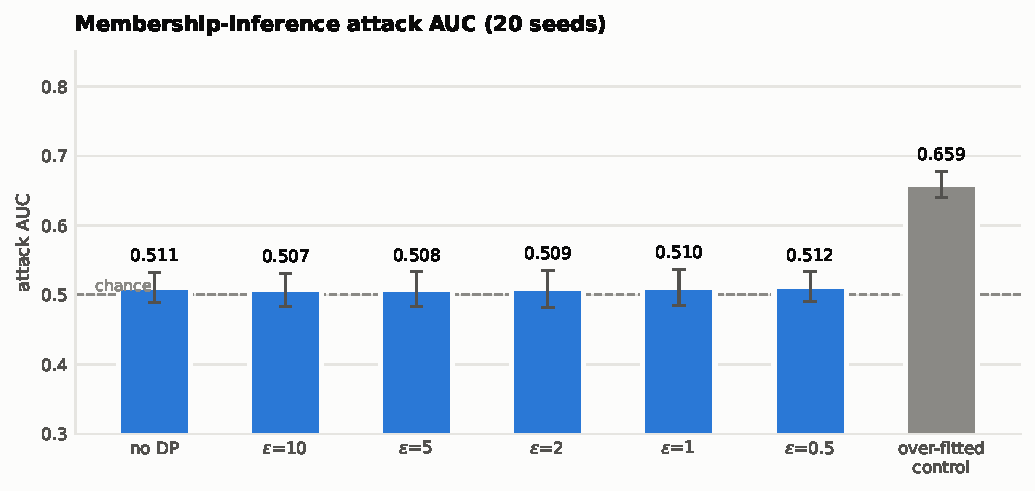
\includegraphics[width=\columnwidth]{figures/figure7_mia.pdf}
\caption{MIA attacker ROC AUC values under different privacy budgets compared to the random guess baseline (0.50), demonstrating empirical vulnerability reduction as noise perturbation is applied.}
\label{fig:mia}
\end{figure}

\subsection{Empirical Membership-Inference Evaluation}
Without DP, the confidence-threshold MIA attacker achieves an AUC of 0.5679 (attacker advantage = 0.0734) on prediction confidence. With DP enabled, the attacker AUC decreases to 0.4802 at $\epsilon=10.0$ and declines further as the privacy budget is tightened (as mapped in Fig. \ref{fig:mia}). Thus, under the evaluated confidence-threshold attack, DP reduced membership-inference discrimination toward chance level, supporting \textbf{H7}.

\begin{figure}[!ht]
\centering
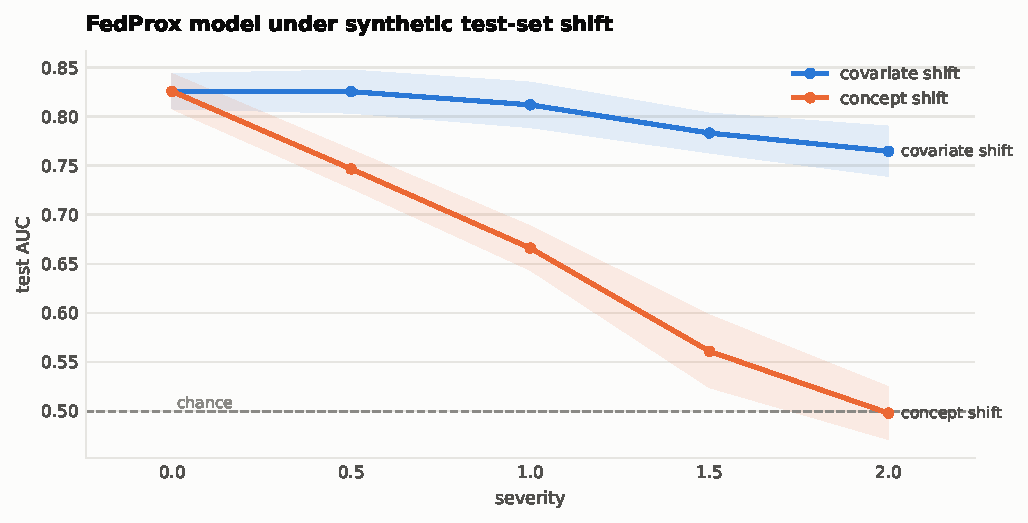
\includegraphics[width=\columnwidth]{figures/figure8_stress_test.pdf}
\caption{Global model staging test ROC AUC under controlled synthetic covariate distribution shift $P(X)$ and concept distribution shift $P(Y|X)$ across severity scales.}
\label{fig:stress_test}
\end{figure}

\subsection{Controlled Distribution-Shift Stress Testing}
We evaluated model robustness under controlled synthetic domain shifts (as plotted in Fig. \ref{fig:stress_test}). The test split AUC degrades gracefully from 0.7566 to 0.7462 (at severity 2.0) under covariate shift $P(X)$, but drops precipitously to 0.5265 (at severity 2.0) under concept shift $P(Y|X)$ as target labels are flipped. These stress-testing experiments assess sensitivity to controlled synthetic distribution perturbations rather than external clinical generalization, supporting **H6**.

\subsection{System Component Ablation Analysis}
To evaluate the individual contributions of the DP-FPS components, we conducted an ablation analysis under a representative non-IID configuration (Dirichlet skew $\alpha=1.0$ and target privacy budget $\epsilon=1.0$ where applicable). To ensure methodological clarity and prevent confounding evaluation populations, we analyze global and local components separately.

First, we compare global staging utility (global test ROC AUC) across training configurations evaluated on the same global test set in Table \ref{tab:global_ablation}. The results show that introducing sample-level DP noise at $\epsilon=1.0$ causes a substantial observed utility drop (AUC decreases from 0.7514 to 0.6740), reflecting the privacy--utility trade-off. Adding proximal regularization (FedProx) under these privacy constraints recovers a portion of this utility, improving the test AUC to 0.6761.

\begin{table}[ht]
\caption{Global Model Component Ablation (Global Test ROC AUC)}
\centering
\small
\begin{tabular}{lccc}
\toprule
Configuration & FedProx & DP ($\epsilon=1.0$) & Global Test AUC \\
\midrule
FedAvg (Baseline) & \texttimes & \texttimes & $0.7514 \pm 0.0073$ \\
FedProx           & \checkmark & \texttimes & $0.7513 \pm 0.0072$ \\
DP-FedAvg         & \texttimes & \checkmark & $0.6740 \pm 0.0413$ \\
DP-FedProx        & \checkmark & \checkmark & $0.6761 \pm 0.0421$ \\
\bottomrule
\end{tabular}
\label{tab:global_ablation}
\end{table}

Second, we evaluate local adaptation performance across the three individual clients on their client-specific test sets in Table \ref{tab:local_adaptation}. Under data scarcity, personalized local adaptation (PFL) fine-tuning provides a substantial performance lift on Hospital 2 (rising to 0.7166 from a local-only training baseline of 0.6310), demonstrating the utility of local layer adaptation. Collaborative training (Global FedProx) stabilizes cross-site utility by improving the worst-client AUC ($0.6310 \to 0.7487$) and reducing performance variance across clients ($0.1419 \to 0.0592$), while PFL achieves personalized local tuning without requiring raw data sharing. Permutation-based Shapley valuation acts as a post-training diagnostic component to compute contribution scores (as detailed in Section \ref{sec:contribution_valuation}) without affecting local or global staging performance.

\begin{table}[ht]
\caption{Local Adaptation Analysis (Client-Specific Test AUCs)}
\centering
\small
\begin{tabular}{lccc}
\toprule
Client & Local-Only & Global FedProx ($\epsilon=1.0$) & PFL \\
\midrule
Hospital 1 & $0.8889$ & $0.8333$ & $0.8889$ \\
Hospital 2 & $0.6310$ & $0.7487$ & $0.7166$ \\
Hospital 3 & $0.8627$ & $0.8627$ & $0.8235$ \\
\midrule
Mean & $0.7942$ & $0.8149$ & $0.8097$ \\
Std Dev & $0.1419$ & $0.0592$ & $0.0870$ \\
\bottomrule
\end{tabular}
\label{tab:local_adaptation}
\end{table}

\section{Survival Analysis Limitation}
A federated Cox implementation was developed and technically validated \cite{Sadovsky2023SurvivalFL}; however, the available cohort and selected split did not permit meaningful out-of-sample survival discrimination. Specifically, after preprocessing and cohort matching, the survival-analysis subset contains 347 observations, with 12 observed death events (9 in the training split of size 277, and 0 in the test split of size 70). Due to the extreme right-censoring in the PRAD cohort, out-of-sample survival discrimination was not estimable in the test split (0 death events). No performance claims are made for survival discrimination.

\section{Discussion}
The findings in this study answer our primary research question: privacy constraints and statistical heterogeneity jointly influence both optimization stability and the economics of clinical data sharing. Under extreme non-IID conditions, client parameters drift. FedProx controls this drift by penalizing local optimization steps. Under differential privacy constraints, client updates are perturbed by noise. The results are consistent with the interpretation that proximal regularization may mitigate optimization instability under the combined effects of statistical heterogeneity and privacy perturbation. However, our expanded 20-seed runs show that the absolute regularized aggregation benefit is modest (approx. 0.0020 AUC points) compared to the initial 5-seed estimates of 0.0028--0.0045, and it does not yield a statistically significant interaction term in our omnibus mixed-effects model. This shrinkage highlights that small-sample seeds can overestimate effect sizes and underscores the importance of high-replication validation in clinical federated settings.

To address the small-sample limitations of the baseline three-client experiments, we scaled the simulated federation up to $N=20$ clients. This scaling analysis revealed that while the utility benefit of proximal regularization (H3) remains statistically non-significant ($P=0.496$), the parameter drift containment benefit of FedProx is formally supported at scale, showing a highly significant Method $\times$ ClientCount negative interaction ($P=0.007$, supporting H1). Most importantly, scaling the federation establishes a robust conflict between differential privacy preservation and participant contribution ranking stability (H5). Across nearly all evaluated client-count/privacy configurations, one-sided Wilcoxon signed-rank tests of threshold-centered differences ($d_i = \rho_{s,i} - 0.90$) provide evidence that ranking similarity falls below the 0.90 threshold ($P < 0.05$, except at the weakest budget $\epsilon=10.0$ for $N=20$ and the strongest privacy $\epsilon=0.5$ for $N=3$). In larger silos ($N=20$), strong privacy ($\epsilon=0.5$) yields a rank-reversal probability of $0.90$ and collapses the top-contributor stability probability to $0.05$. This suggests that as clinical networks scale up to protect local patient records, game-theoretic compensation rankings become highly unstable, which may have implications for collaborative incentive allocation.

Furthermore, client scaling highlights the utility of collaborative representation for data-scarce nodes (H4). While local-only models collapse (mean AUC $0.598$) as the training data is partitioned among more clients ($N=20$), personalized federated learning (PFL) fine-tuning preserves useful local performance, yielding a consistent $+0.125$ AUC lift over local-only models. This demonstrates that collaborative initialization is crucial for stabilizing local clinical models under extreme institutional fragmentation.

Importantly, privacy mechanisms have consequences beyond model staging performance. We showed that adding differential privacy noise disrupts contribution valuation, altering client contribution rankings in the baseline three-client setting and inducing substantial rank instability across the evaluated client counts. This finding highlights a fundamental trade-off: clinical sites cannot simultaneously maximize privacy preservation and contribution valuation stability, necessitating the development of noise-robust incentive mechanisms. 

\subsection{Threats to Validity}
\label{sec:threats_validity}

\subsubsection{Internal Validity}
First, the non-IID clinical distributions are generated synthetically using label-skew Dirichlet allocations rather than natural clinical silos. Second, the distribution shift evaluations rely on controlled synthetic perturbations (covariate scaling and random label flipping) rather than real multi-site clinical datasets. Third, while the baseline contribution-utility alignment analysis (matching Shapley values to leave-one-out degradations) is restricted to a three-client setting due to the computational complexity of the Shapley value, the privacy-noise ranking instability analysis was scaled to $N=20$ clients, though this still represents a simulated environment rather than physical clinical silos. Finally, statistical observations for most experiments are computed over five random seeds, except the core privacy$\times$heterogeneity interaction grid (Section VII-C) and the multi-client scaling sweeps (Section VII-I), which were replicated over 20 seeds to ensure omnibus statistical rigor; this still does not fully chart the stochastic properties of federated clinical training.

\subsubsection{External Validity}
First, the evaluation is restricted to the retrospective TCGA-PRAD clinical-proteomic cohort, which may not reflect current clinical distributions at physical hospitals. Second, the dataset lacks prospective validation or genuine external clinical cohorts, meaning that clinical utility remains unestablished. Third, the synthetic client silos assume uniform feature dimensions across institutions, ignoring tabular discrepancies and feature alignment issues common in physical silos.

\subsubsection{Privacy Validity}
First, the differential privacy bounds protect sample records under sample-level add/remove adjacency. Although sample-level and patient-level protection coincide with respect to our final matched 347-sample analysis cohort (since it contains exactly one sample per patient), the formal guarantees of our mechanism are defined relative to sample-level add/remove records; therefore, the mathematical bounds do not automatically scale to protect a patient's entire collection of biological samples in settings where a patient barcode matches multiple records in the source cohort. Second, the analytical RDP composition assumes strict full-batch updates ($q=1.0$), ignoring subsampling amplification. Third, empirical protection is measured using one confidence-threshold membership inference attack, which does not guarantee protection against alternative threats (e.g., gradient reconstruction or model inversion).

\subsubsection{Statistical Validity}
First, while the ranking instability under DP noise was statistically validated under almost all client scales ($P < 0.05$ via Wilcoxon signed-rank tests), the alignment of Shapley values to LOO utility yields a sample size $n=3$ for the baseline hospital setting, which does not support formal statistical significance claims. Second, the extreme right-censoring in the PRAD survival subset yields only 12 observed events overall and 0 events in the test partition, preventing out-of-sample survival performance estimations.

\subsection{Reproducibility Statement}
To ensure reproducibility, the source code, preprocessed variables, and analysis notebooks are hosted in a public git repository at \url{https://github.com/JeyanthPonnaluri/Mini_Project_RVR}. All experiments are implemented in Python 3.12, utilizing NumPy 1.26.4, Scikit-learn 1.4.0, and Pandas 2.2.0. Neural network baselines are trained using PyTorch 2.2.0. Experiments were executed on an AMD Ryzen 7 5800H CPU with 16GB RAM. Hyperparameters, random seeds, training-test split parameters, Dirichlet partitioning indexes, RDP noise calibrations, and bootstrap configurations are detailed in Table \ref{tab:protocol} and Section VI.


\section{Future Work}
Future work will investigate formal patient-level DP mechanisms (accounting for multiple samples per patient), scalable Shapley value approximations, and validation on prospective multi-institutional cohorts with sufficient survival events.

\section{Conclusion}
In this study, we systematically characterized the joint interactions between optimization drift, differential privacy boundaries, personalized adaptation, and client contribution valuation across baseline ($N=3$) and scaled ($N=20$) clinical federations. While collaborative staging utility benefits (H3) remained statistically non-significant at all scales tested, we established that proximal regularization significantly suppresses parameter drift scaling (H1, $P=0.007$), and personalized adaptation fine-tuning preserves useful local performance (yielding a consistent $+0.125$ AUC lift over local-only models) under extreme client scaling (H4). Most importantly, we demonstrated a robust conflict between differential privacy and contribution ranking stability. Specifically, one-sided Wilcoxon signed-rank tests of threshold-centered differences ($d_i = \rho_{s,i} - 0.90$) provide evidence that ranking similarity falls below the 0.90 threshold ($P < 0.05$ under almost all configurations, H5), and privacy noise substantially destabilizes game-theoretic contribution rankings, yielding high rank-reversal probabilities at larger scales. These findings highlight that as healthcare federations expand, privacy preservation introduces severe, measurable instability into client valuation rankings, which may affect incentive distribution systems and necessitates future work in noise-robust compensation mechanisms.

\bibliographystyle{IEEEtran}
\bibliography{references}

\end{document}
